% lint-skip: 未完成ステータス（figure/table caption 未対応，人手チェック時に解消予定）
\documentclass[../../main.tex]{subfiles}
\begin{document}

\begin{flushright}
  \footnotesize\textit{【自動文字起こし・要確認】}
\end{flushright}

[解]

\paragraph{(1)}

\begin{figure}[htb]
  \centering
  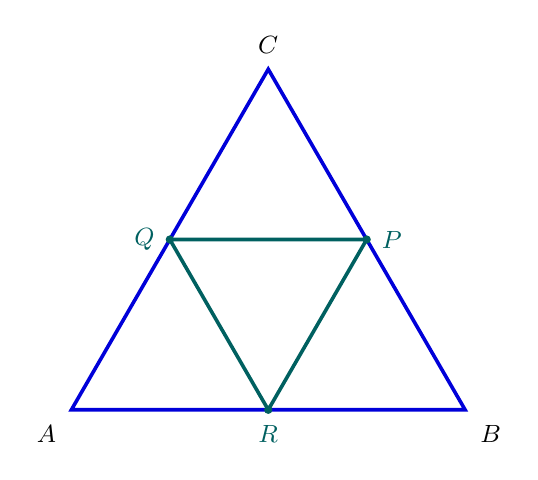
\begin{tikzpicture}[x=1.25cm, y=1.25cm,
    every node/.style={font=\small}]
    % Symmetric case a=b=c: all three feet are side midpoints.
    \coordinate (A) at (-2,0);
    \coordinate (B) at (2,0);
    \coordinate (C) at (0,3.46);
    \coordinate (R) at (0,0);
    \coordinate (P) at (1,1.73);
    \coordinate (Q) at (-1,1.73);
    \draw[line width=1.3pt, blue!85!black]
    (A) -- (B) -- (C) -- cycle;
    \draw[line width=1.3pt, teal!75!black]
    (Q) -- (P) -- (R) -- cycle;
    \foreach \T in {P,Q,R} {
      \fill[teal!75!black] (\T) circle (1.5pt);
    }
    \node[below left=2pt] at (A) {$A$};
    \node[below right=2pt] at (B) {$B$};
    \node[above=2pt] at (C) {$C$};
    \node[below=2pt, teal!75!black] at (R) {$R$};
    \node[right=2pt, teal!75!black] at (P) {$P$};
    \node[left=2pt, teal!75!black] at (Q) {$Q$};
  \end{tikzpicture}
  \caption{$\triangle ABC$ の各辺上にある垂足 $P,Q,R$（対称な例）}
\end{figure}
\begin{figure}[htb]
  \centering
  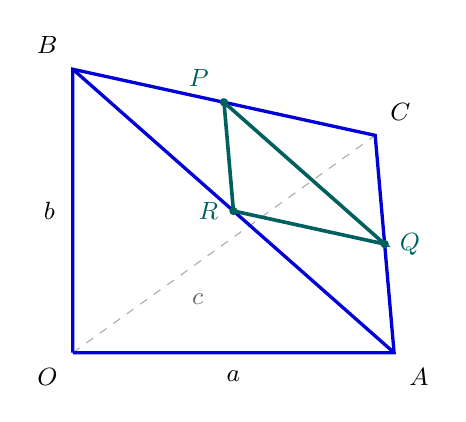
\begin{tikzpicture}[x=1.2cm, y=1.2cm,
    every node/.style={font=\small}]
    % A projected view of three perpendicular spatial edges OA, OB, OC.
    \coordinate (O) at (0,0);
    \coordinate (A) at (3.4,0);
    \coordinate (B) at (0,3);
    \coordinate (C) at (3.2,2.3);
    \coordinate (P) at (1.6,2.65);
    \coordinate (Q) at (3.3,1.15);
    \coordinate (R) at (1.7,1.5);
    \draw[dashed, gray!65] (O) -- (C);
    \draw[line width=1.2pt, blue!85!black]
    (O) -- (A) -- (C) -- (B) -- (O);
    \draw[line width=1.2pt, blue!85!black] (A) -- (B);
    \draw[line width=1.3pt, teal!75!black]
    (P) -- (Q) -- (R) -- cycle;
    \foreach \T in {P,Q,R} {
      \fill[teal!75!black] (\T) circle (1.5pt);
    }
    \node[below left=2pt] at (O) {$O$};
    \node[below right=2pt] at (A) {$A$};
    \node[above left=2pt] at (B) {$B$};
    \node[above right=2pt] at (C) {$C$};
    \node[above left=2pt, teal!75!black] at (P) {$P$};
    \node[right=2pt, teal!75!black] at (Q) {$Q$};
    \node[left=2pt, teal!75!black] at (R) {$R$};
    \node[below=3pt] at (1.7,0) {$a$};
    \node[left=3pt] at (0,1.5) {$b$};
    \node[below right=2pt, gray!80!black] at (1.1,0.79) {$c$};
  \end{tikzpicture}
  \caption{互いに直交する $OA,OB,OC$ と三角形 $PQR$ の位置関係}
\end{figure}

底面を各々$\triangle ABC, \triangle PQR$とみると，高さ一定だから
\[ V_{OPQR} : V_{OABC} = \triangle PQR : \triangle ABC \quad \cdots \text{①} \]
である．三角形の相似から
\[ |AQ| : |AO| = a : \sqrt{a^2+c^2} \therefore |AQ| = \dfrac{a^2}{\sqrt{a^2+c^2}} \]
同様にして
\[ |AR| = \dfrac{a^2}{\sqrt{a^2+b^2}}, \quad |BP| = \dfrac{b^2}{\sqrt{b^2+c^2}} \]
だから $\triangle ABC$の面積を1として
\begin{align}
  \triangle ARQ &= \dfrac{a^2}{a^2+b^2} \cdot \dfrac{a^2}{a^2+c^2} \\
  \triangle BPR &= \dfrac{b^2}{a^2+b^2} \cdot \dfrac{b^2}{b^2+c^2} \\
  \triangle PCQ &= \dfrac{c^2}{b^2+c^2} \cdot \dfrac{c^2}{a^2+c^2}
\end{align}
だから
\begin{align}
  \triangle PQR &= 1 - \dfrac{a^4(b^2+c^2) + b^4(c^2+a^2) + c^4(a^2+b^2)}{(a^2+b^2)(b^2+c^2)(c^2+a^2)} \\
  &= \dfrac{2a^2b^2c^2}{(a^2+b^2)(b^2+c^2)(c^2+a^2)}
\end{align}
より ①から
\[ V_{OPQR} : V_{OABC} = 2a^2b^2c^2 : (b^2+c^2)(c^2+a^2)(a^2+b^2) \]

\paragraph{(2)}

(1)から
\[ \dfrac{2a^2b^2c^2}{(b^2+c^2)(c^2+a^2)(a^2+b^2)} \le \dfrac{1}{4} \]
\[ 8ABC \le (B+C)(C+A)(A+B) \quad \cdots \text{②} \]
($A=a^2, B=b^2, C=c^2$ とおいた)

を示せばよい．A,B,CからAM-GMより
\[ B+C \ge 2\sqrt{BC} > 0 \]
などとした3式をかけあわせると ②は示される(終)

\end{document}
